\documentclass[a4paper,12ptc]{jsarticle} %文字サイズは変えても良い
\usepackage[dvipdfmx]{graphicx}
\usepackage{amssymb, amsmath}
\usepackage{url}
\usepackage{tikz}  
\usetikzlibrary{decorations.pathreplacing,calligraphy}
\usepackage{float}
\usepackage{setspace}
\usepackage[top=30truemm,bottom=30truemm,left=25truemm,right=25truemm]{geometry} % ページの設定
\pagestyle{empty} %ページ番号なし
%\setlength{\headheight}{0truemm}
%\setlength{\parindent}{1zw}
\makeatletter
\def\section{\@startsection {section}{1}{\z@}{.7ex plus .2ex minus .2ex}{.1 ex plus 1.2ex}{\normalsize\bf}}
\makeatother
\setstretch{0.9}

\newcommand{\normal}{\mathcal{N}}
\newcommand{\exponential}{\mathcal{E}}
\newcommand{\truncnorm}{\mathcal{TN}}
\newcommand{\gam}{\mathcal{G}}
\newcommand{\C}{C}
\newcommand{\one}{1\!\!1}

\begin{document}
%\twocolumn[ 
\begin{center}
{\bf \Large 同時テンソル分解の拡張による医学データの統合}
\vspace{0.3em}
\begin{tabular}{rl}
\vspace{-0.1em} \bf 東京医科歯科大学難治疾患研究所 &  \bf 阿部興 \\
\vspace{-0.1em} \bf 名古屋大学大学院医学系研究科/東京医科歯科大学難治疾患研究所 &  \bf 島村徹平\\
\end{tabular}
\vspace{0.5em}
\end{center}
%]
\vspace{\baselineskip}

%\maketitle
\section{はじめに}
生命科学の分野においては, 生体内に存在する分子を網羅的に観測することが可能になった. 
これらは考察される対象の分子(これをモダリティと呼ぶことにする)が遺伝子であればゲノミクス,転写物であればトランスクリプトミクス,代謝物であればメタボロミクスといった様々な分野があり, 総称としてはオミクス(omics)データと呼ばれる. 中でも, ある1つのサンプルに対し複数のモダリティを計測するマルチオミクスデータは, 生命現象についての豊富な情報を持つものとして注目されている. 一方で, マルチオミクスデータをどのように分析すべきかは未だ議論が続いている.

複数のモダリティをまたいだ分析を難しくする原因の一つとして, 計測に関わる現実的な制約のために, 対応があるサンプルとないサンプルが混在する semi-paired なデータが多く見られることがあげられる. また, あるモダリティは計数データ, あるモダリティは連続値のデータといった形で, データの分布が大きく変わることも統一的な分析を難しくしている.

Abe \& Shimamura (2023) ではNMFを拡張し, 多次元のデータを柔軟に分析するモデルとして,  unified non-negative matrix factorization (UNMF) を提案した. しかし, UNMFはポアソン分布を仮定していたため, 本報告ではより幅広いクラスのデータを柔軟にあつかえる枠組みについて考察する.

%\section{}

\section{モデルと推定アルゴリズム}
\subsection{概要}
確率モデルとしての定式化の前に, まず我々が提案する手法の概要を, そのモチベーションが理解できるように述べたい. 簡単のため, 3階のテンソル $Y=(y_{i,j,k})$を考える. ここでは単に添字($i,j,k$)を定めたとき値が1つに決まるような変数(多次元配列)という意味でテンソルという語を用いる. さらに $\mathrm(vec)(Y)$ を適当な順番で $Y$ のすべての要素をベクトルに配置する作用素とする. 
CP分解(正準分解や並行因子分解とも呼ばれる)では各要素が次を満たすような行列 $V^{(k)}$ ($k=1,2,3$)を作る.
\begin{equation*}
y_{ijk} \approx \sum_{r}v_{ir}^{(1)} v_{jr}^{(2)} v_{kr}^{(3)}. 
\end{equation*}
この式は次のように書き換えられる:
\begin{equation}
y_{n} \approx \sum_{r}\prod_{d=1}^D v_{dr}^{x_{nd}} \label{eq_approx}
\end{equation}
ここで
\begin{align*}
V=(v_{dl})=\begin{pmatrix}
v^{(1)}\\
v^{(2)}\\
v^{(3)}
\end{pmatrix}
\end{align*}
and $x_{nd} \in \{0, 1\}$ is one-hot encoded matrix $(\xi_1, \xi_2, \xi_3)$. 
This representation not conflict the cases that even when the number of subscripts increases or duplicate, even when there are missing values. 
This fact means our methods can be easily handle semi-paired samples with multi-modal (see Fig. \ref{fig_mosaic}).

また交互作用項を考えることは
\begin{align*}
y_{ijk} &\approx \sum_{r}\prod_{d=1}^D v_{dr}^{x_{nd}} \\
&=\begin{cases}
\sum_{r}v_{ijr}^{(1)}v_{jr}^{(2)}v_{kr}^{(3)} & \mbox{when $X$ consisiting from $\xi_1 \cdot \xi_2$, $\xi_2$, and $\xi_3$}\\
\sum_{r}v_{ir}^{(1)} v_{jkr}^{(2)} v_{kr}^{(3)} & \mbox{when $X$ consisiting from $\xi_1$, $\xi_2 \cdot \xi_3$, and $\xi_3$}\\
\end{cases}
\end{align*}
このことも semi-paired なデータの分析にとって有益である. 例えば, 行の軸では対応があるが列の軸では対応のない行列を分析するときは, 列ダミーとモダリティの交互作用項を考える.

\begin{figure}
    \centering
    \begin{tabular}{c|c}
    \footnotesize (a)
    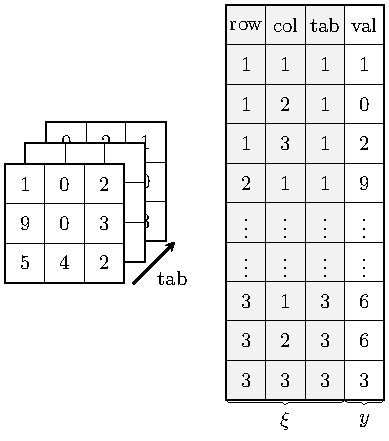
\includegraphics[width=0.2\textwidth]{img/threeway.pdf} &
    \footnotesize (b)
    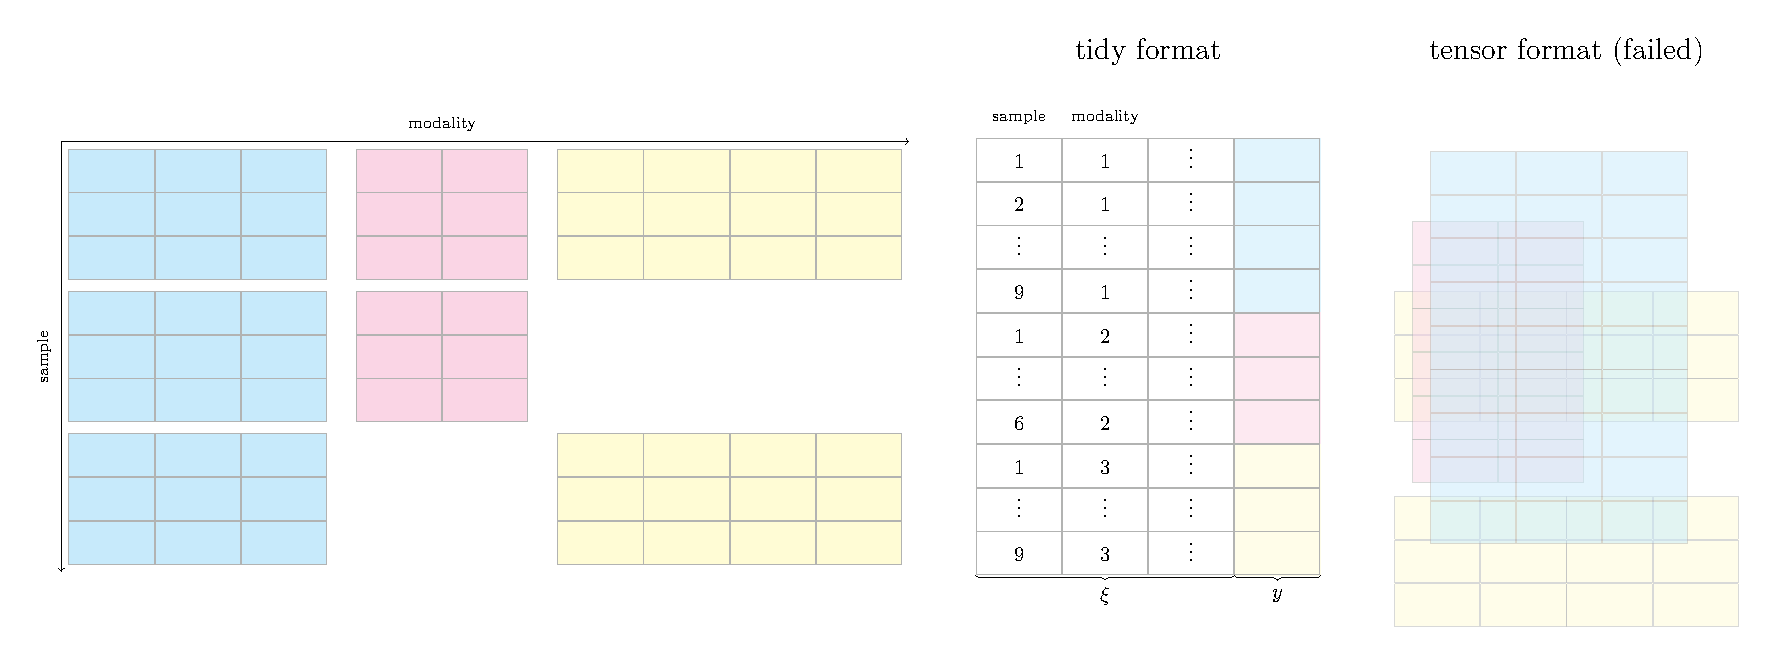
\includegraphics[width=0.7\textwidth]{img/mosaic.pdf} 
    \end{tabular}
    \caption{Conceptual view for semi-pared data integration. (a)Arbitrary $m$-way tensor can be replanted as tidy-format. The left matrices and the right tidy data structure are equivalent to each other. The all of the index set $\xi$ is map to dummy encoded vectors $x_n$ (b) Data that is difficult to represent as a multidimensional array, can also be stored as tidy-format. White cell indicates a missing value.}
    \label{fig_mosaic}
\end{figure}

\subsection{モデル}

\begin{align}
y_n & \sim \normal\left(y_n \mid \sum_{l=1}^L \prod_{d=1}^D v_{dl}^{x_{nd}}, \lambda^{-1}\right) \label{eq_mod1}\\
v_{dl} & \sim \normal(v_{dl} | 0,\tau^{-1}) \label{eq_prior1}\\
\lambda & \sim \gam(\lambda | a,b) \nonumber
\end{align}
ここで $V=(v_{dl})$ は $D \times L$  行列, 
%where $V$ is a $(D \times L)$ matrix with $v_{dl}$ as the $(d,l)$-th element and $\gam(x|a,b)$ is gamma distribution with shape and rate parameters $a$ and $b$, respectively.


\paragraph{Non-negative constraint}
For realizing non-negative constraint,  use the following truncated normal prior distribution, instead of the normal prior distribution in Eq.\ref{eq_prior1}:
\begin{equation}
v_{dl} \sim \truncnorm(v_{dl} | 0, \tau^{-1}) \label{eq_prior2}
\end{equation}
where $\truncnorm(x | \mu, \sigma^2)$ is left truncated normal distribution (truncated at 0) with the mean parameter $\mu$ and the variance parameter $\sigma^2$, respectively. 
Note that truncated normal density can be written as follows:
\begin{equation*}
   \truncnorm(x | \mu, \sigma^2) \propto    \normal(x | \mu, \sigma^2) \one(x) 
\end{equation*}
where $\one(x)$ is indicator function as follows:
\begin{align*}
    \one(x)=\begin{cases} 1 & x>0\\
    0 &x \leq 0\end{cases}.
\end{align*}

In principle, $v_dl$, which is constrained to be non-negative, can be selected for each subscript $d$, but in our implementation, only $d$ specified as the first variable allows negative values (\verb|constraint = SN| mode in the package \verb|moltenCP|). 
This is to avoid complicated interpretations of $(-1)\times(-1)$. Depending on the order on the columns, we can choose a variable which takes a negative value.

\paragraph{Auxiliary variables}
When the support of the distribution of $y$ is clearly restricted, we introduce the following auxiliary variable $z_n$ in the model of Eq.\ref{eq_mod1}.
\begin{equation}
    y_n = A(z_n), \quad z_n \sim \mathcal{N}\left(\sum_{l=1}^L \prod_{d=1}^Dv_{dl}^{x_{nd}}, \lambda^{-1}\right).
\end{equation}
The function $A(x)$  can be chosen as follows:
\begin{itemize}
\item If the observed $y_n$ takes continuous values with no exact zeros, we would use an identity function 
$$
A(x)=x.
$$
    \item 
$y_n$ is non-negative:
$$
A(x)=\begin{cases}x, &x>0\\0 &x\leq 0\end{cases}.
$$
\item
$y_n$ is binary(0 or 1):
$$
A(x)=\one(x).
$$
\item
$y_n$ is non-negative integer:
$$
A(x)=\begin{cases}\lceil x\rceil, & x>0\\0 &x\leq 0\end{cases}.
$$
\end{itemize}
Utilizing the normal density as the observation model implies using a symmetric loss function to evaluate the fit.
When the analyst already knows that there are no negative values in the observed data (for example, in the case of weight, length, or count data), predicting 0 as 1 is not the same as predicting it as -1.
In these cases, it makes sense to change the support of the model's density function.

When we want to analyze multiple matrices (tensors) simultaneously, the data distribution may vary depending on the modality. 
We consider this issue in the next.

\paragraph{Multi-modal analysis} Next, we consider that multiple modes and we want to change the distribution for each mode $m$. The observation model in Eq.\ref{eq_mod1} is switched to following Eq.\ref{eq_mod2}  
\begin{equation}
    y_{n} = A_{m(n)}(z_{n}), \quad z_{n} \sim \mathcal{N}\left(\sum_{l=1}^L \prod_{d=1}^Dv_{dl}^{x_{ndm}}, \lambda^{-1}_m\right) \label{eq_mod2}    
\end{equation}
where $m(n)$ is a function which maps index $n$ to mode $m(n)$. 

\paragraph{Offset factor}
We often want to correct the observed $y_n$ using the known ``weight" $w_n$; such as, the size when the library size is different, or the time when the time required for measurement is different.
In such case, we can address this by making a simple change to Eq.\ref{eq_mod2} as following:
\begin{equation}
y_n = A_{m(n)}(z), \quad z_n\sim \normal\left(y_n \mid w_n \sum_{l=1}^L \prod_{d=1}^D v_{dl}^{x_{nd}}, \lambda^{-1}\right).\label{eq_mod_off}
\end{equation}
When the all elements of $w=(w_1, \ldots , w_N)$ is 1, this observation model is equivalent to Eq.\ref{eq_mod2}.

\paragraph{Log-joint density}
In above mentioned settings, the log likelihood $\ell(v_{dl})$ is represented as following:
\begin{align*}
& \ell(v_{dl}) =\sum_{n=1}^{N} \log p(z|V, X, w)\\
&= \sum_{n=1}^{N}\left(-\frac{\lambda}{2}\left\{ z_n -\sum_{l=1}^L\prod_{d=1}^D v_{dl}^{x_{nd}} \right\}^2\right)+ \C\\
&= -\sum_{m=1}^M\frac{h_{dlm}}{2}\left(v_{dl}^2-2v_{dl}\frac{\eta_{dlm}}{h_{dlm}}\right) +C,
\end{align*}
where $C$ is constant term which not depends on $v_{dl}$, and let $\eta_{dlm}$ and $h_{dlm}$ be as follows;
\begin{align}
\eta_{dlm} &= \sum_n x_{ndm} \prod_{d' \neq d} v_{dl}^{x_{ndm}}\left( z_{nm} - \sum_{l'\neq l} \prod_{d' \neq d} v_{dl}^{x_{ndm}} \right) \label{eq_eta}\\
h_{dlm} &= \sum_n \lambda_m x_{ndm} \prod_{d' \neq d} v_{dl}^{2x_{ndm}}. \label{eq_h}
\end{align}

In the next subsection, we derive the variational EM algorithm from this logarithmic joint density.

\subsection{Estimation procedure}
\label{est_sec}
\subsubsection{Variationl EM algorithm}
This subsection we derived estimator of the latent variables based on the variationl EM algorithm\cite{Jordan}. 
Using mean-field approximation (i.e. suppose that variational posterior distributions $q(v_{dl})$ and $q(\lambda$ are independent) and let $\langle x \rangle$ be the expectation of $x$ under the variational posterior distribution, we get following variational posterior of $v_{dl}$ as following; 
\begin{align}
q(v_{dl})= \begin{cases}
\normal(\mu_{dl}, \sigma_{dl}) & \mbox{if the prior of $v_{dl}$ is not truncated} \\
\truncnorm(\mu_{dl}, \sigma_{dl}) & \mbox{if the prior of $v_{dl}$ is truncated},     
\end{cases} \label{qv}
\end{align}
where $v_{dl}$ and $\sigma_{dl}$ are defined by
\begin{align*}
\mu_{dl} &=\sum_{m=1}^M \frac{\langle \eta_{dlm} \rangle}{\langle h_{dlm}\rangle+\tau/\langle\lambda_m\rangle},\\
\sigma^2 &=\left(\tau + \sum_{m=1}^M \langle h_{dlm} \rangle \right)^{-1}.
\end{align*}
The variational posterior of $\lambda_{m}$ is,  
\begin{align}
    q(\lambda) = \gam\left(N_m/2 \eta_{dlm}, \left(\sum_m h_{dlm}+\tau\right)/2\right). \label{qlam}
\end{align}
The expectations which used for variational updates are listed as following:
\begin{align*}
\langle v_{dl}\rangle &=\mu_{dl} + \sigma_{dl} \phi(-\mu_{dl}/\sigma_{dl})/\Phi(-\mu_{dl}/\sigma_{dl}),\\
\langle v_{dl}^2 \rangle&=\mu_{dl}^2 + \sigma_{dl}^2 + \mu_{dl} \sigma_{dl} \phi(-\mu_{dl}/\sigma_{dl})/\Phi(-\mu_{dl}/\sigma_{dl}),\\
\langle \lambda_m \rangle &= (N_m \langle \eta_{dlm} \rangle ) / \left(\sum_m \langle h_{dlm} \rangle +\tau\right).
\end{align*}
where $\phi(x)$ and $\Phi(x)$ is standard normal density and distribution function, respectively.

For \textit{local} latent variable $z_n$, we use Monte-Carlo integral, i.e. sample $\tilde z_n$ using variational posterior as follows
\begin{itemize}
\item Rectified
\begin{align}
q(-z_n) = \begin{cases}
    \mathcal{TN}(-z_n|-f_n, \sigma_n^2) & y_n=0,\\
    z_n = y_n \mbox{~with probability 1} & y_n>0
\end{cases}
\end{align}
\item binary
\begin{align}
q(-z_n) = \begin{cases}
    \mathcal{TN}(-z_n|-f_n, \sigma_n^2) & y_n=0,\\
    \mathcal{TN}(z_n|f_n, \sigma_n^2) & y_n=1
\end{cases}
\end{align}
\end{itemize}

The estimation procedure can be briefly summarized as follows:
\begin{itemize}
\item variational E-step: draw $\tilde{z}_n$ for all $n$s
\item variational M-step: update $q(V)$ using Eq.\ref{qv} and update $q(\lambda)$ using Eq.\ref{qlam}
\end{itemize}

The appendix\ref{app_imple} describes some notes for efficient implementation.

\section{シミュレーション}


当日はデータ分析事例をあわせて報告する.

\begin{thebibliography}{9}
\bibitem{AbeShimamura} Abe K \& Shimamura T. (2023). UNMF: A unified non-negative matrix factorization for multi-dimensional omics data. {\em Briefings in Bioinformatics.} (Under Review).
\end{thebibliography}
\end{document}  m 